\section{Image processing and information extraction}\label{sec:improc}

\subsection{Simple calculus with channels}\label{ssec:calculus}

The \application{BandMath} application provides a simple and efficient 
way to perform band operations. The command line application and the 
corresponding Monteverdi module (shown in the section \ref{Band_math module}) 
are based on the same standards. It computes a band wise operation according 
to a user defined mathematical expression. The following code computes the 
absolute difference between first bands of two images:

\begin{verbatim}
otbcli_BandMath -il input_image_1 input_image_2 
                -exp "abs(im1b1 - im2b1)"
                -out output_image
\end{verbatim}

The naming convention "im[x]b[y]" designates the yth band of the xth input image.

The \application{BandMath} application embeds built-in operators and functions 
(listed \href{http://muparser.sourceforge.net/mup_features.html#idDef2}{here}), 
allowing a vast choice of possible operations. 

\subsection{Classification}\label{ssec:classification}

The SVM classification in application framework provides a supervised pixel-wise 
classification chain based on learning from multiple images. It supports huge 
images through streaming and multi-threading.
The classification chain performs a SVM training step based on the intensities 
of each pixel as features. Please note that all the input images must have the 
same number of bands to be comparable.

\subsubsection{Statistics estimation}
In order to make these features comparable between each images, the first step 
is to estimate the input images statistics. These statistics will be used to 
center and reduce the intensities (mean of 0 and standard deviation of 1) of 
samples based on the vector data produced by the user. To do so, the 
\application{ComputeImagesStatistics} tool can be used :

\begin{verbatim}
otbcli_ComputeImagesStatistics -il  list_of_input_images 
                               -out statistics.xml
\end{verbatim}

This tool will compute each band mean, compute the standard deviation based on 
pooled variance of each band and finally export them to an XML file.
The features statistics XML file will be an input of the following tools. 

\subsubsection{Building the training data set}

As the chain is supervised, we need first to build a training set with
positive examples of different objects of interest. This can be done
with Monteverdi Vectorization module
(Fig.\ref{fig:vectoModuleDataSetCreation}). 
These polygons must be save in OGR vector format supported
by GDAL like ESRI shapefile for example.

This operation will be reproduced on each image used as input of the training 
function.

Please note that the positive examples in the vector data should have a ``Class`` 
field with a label value higher than 1 and coherent in each images. 

\begin{figure}
  \center
  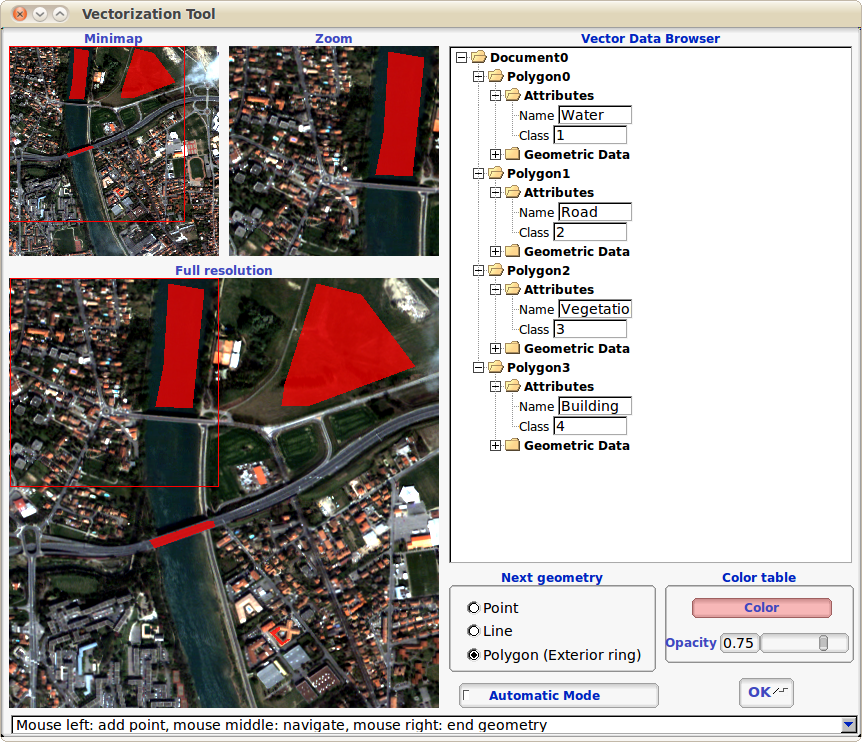
\includegraphics[width=1\textwidth]{../Art/MonteverdiImages/monteverdi_vectorization_module_for_classification.png}
  \itkcaption[GUI of the vectorization module with data for classification chain]{A training data set builded with the vectorization monteverdi module.}
  \label{fig:vectoModuleDataSetCreation}
\end{figure}

You can generate the vector data set with \qgis software for
example and save it in an OGR vector format supported by \gdal (ESRI
sphapefile for example). \app should be able to transform the
vector data into the image coordinate system.

\subsubsection{Performing the learning scheme}

Once images statistics have been estimated, the learning scheme is the following:
\begin{enumerate}
  \item For each input image:
  \begin{enumerate}
    \item Read the region of interest (ROI) inside the shapefile,
    \item Generate validation and training data within the ROI,
    \item Add vectors respectively to the training samples set and the validation 
    samples set.
  \end{enumerate}
  \item Increase the size of the training samples set and balance it by 
  generating new noisy samples from the previous ones,
  \item Perform the learning with this training set
  \item Estimate performances of the classifier on the validation samples set 
  (confusion matrix, precision, recall and F-Score).
\end{enumerate}

These steps can be performed by the \application{TrainSVMImagesClassifier} 
command-line using the following:

\begin{verbatim}
otbcli_TrainSVMImagesClassifier -io.imstat  images_statistics.xml 
                                -io.il  list_of_input_images 
                                -io.vd  list_of_positive_examples_shapefiles
                                -io.out model.svm
\end{verbatim}

Optionnal groups of parameters are also available (see application help for 
more details):
\begin{itemize}
\item \verb?-elev? Handling of elevation (DEM or average elevation)
\item \verb?-sample? Group of parameters for sampling
\item \verb?-svm? Group of parameters for SVM
\end{itemize}

\subsubsection{Validating the classification model}
It is also possible to estimate the performance of the SVM model with a 
new validation sample set and another image with the 
\application{ValidateSVMImagesClassifier} application. It will compute 
the global confusion matrix and precision, recall and F-score of each 
class based on the \href{http://www.orfeo-toolbox.org/doxygen-current/classotb_1_1ConfusionMatrixCalculator.html}{ConfusionMatrixCalculator} 
class.

\begin{verbatim}
otbcli_ValidateSVMImagesClassifier -imstat  images_statistics.xml
                                   -svm model.svm
                                   -il  input_image_list
                                   -vd  list_of_positive_examples_shapefiles
\end{verbatim}

You can save these results with the option -out output filename. 
%You can also set a DEM repository (-dem) to keep the vectordata reprojection accurate.

\subsubsection{Using the classification model} 
Once the classifier has been trained, one can apply the model to classify 
pixel inside defined classes on a new image using the 
\application{ImageSVMClassifier} application:

\begin{verbatim}
otbcli_ImageSVMClassifier -imstat  images_statistics.xml
                          -svm model.svm 
                          -in  input_image
                          -out labeled_image
\end{verbatim}

You can set an input mask to limit the classification to the mask area with 
value \textgreater 0.

\subsubsection{Fancy classification results}

Color mapping can be used to apply color transformations on the final 
graylevel label image. It allows to get an RGB classification map 
by re-mapping the image values to be suitable for display purposes.
One can use the \application{ColorMapping} application. This tool will 
replace each label with an 8-bits RGB color specificied in a mapping 
file. The mapping file should look like this :

\begin{verbatim}
# Lines beginning with a # are ignored
1 255 0 0
\end{verbatim}

In the previous example, 1 is the label and 255 0 0 is a RGB color 
(this one will be rendered as red). To use the mapping tool, enter 
the following :

\begin{verbatim}
otbcli_ColorMapping -in  labeled_image 
                    -out color_image
                    -method custom
                    -method.custom.lut  mapping_file
\end{verbatim}

Other look-up tables (LUT) are available : standard continuous LUT, 
optimal LUT, and LUT computed over a support image. 

\subsubsection{Example}
We take 4 classes: water, roads, vegetation and buildings with red roof.
Data is available in the OTB-Data 
\href{http://hg.orfeo-toolbox.org/OTB-Data/file/0fed8f4f035c/Input/Classification}{repository} 
and this image is produced with the commands inside this 
\href{http://hg.orfeo-toolbox.org/OTB-Applications/file/3ce975605013/Testing/Classification/CMakeLists.txt}{file}. 

\begin{figure}[!h]
  \center
  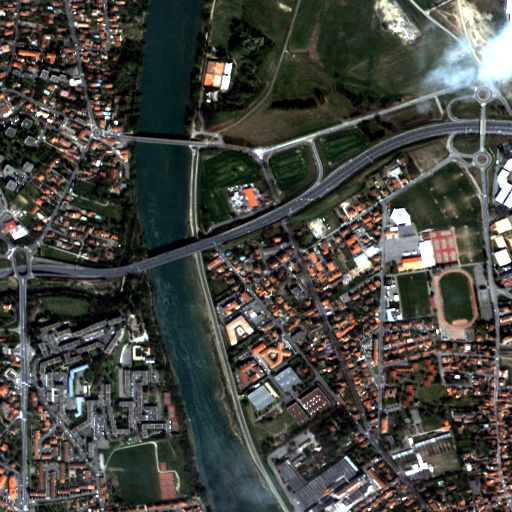
\includegraphics[width=0.3\textwidth]{../Art/MonteverdiImages/classification_chain_inputimage.jpg}
  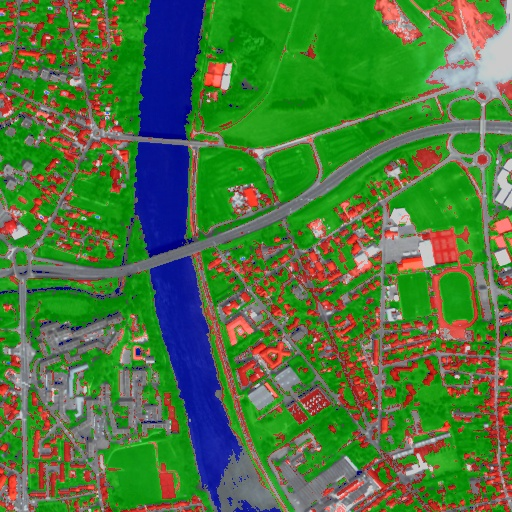
\includegraphics[width=0.3\textwidth]{../Art/MonteverdiImages/classification_chain_fancyclassif_fusion.jpg}
  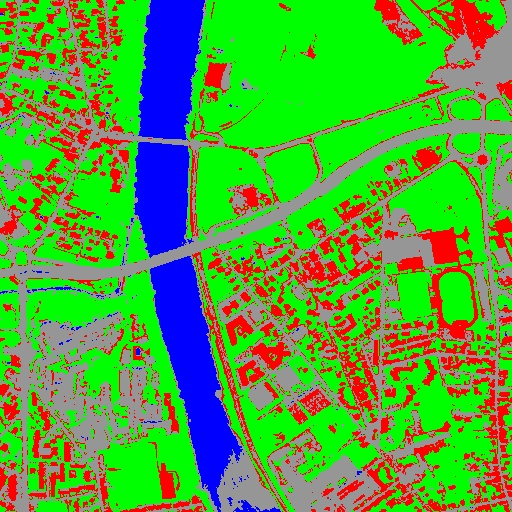
\includegraphics[width=0.3\textwidth]{../Art/MonteverdiImages/classification_chain_fancyclassif.jpg}
  \itkcaption[ExampleSVMCalssif]{From left to right: Original image, 
    result image with fusion (with monteverdi viewer) of original 
    image and fancy classification and input image with fancy color 
    classification from labeled image.}
  \label{fig:MeanShiftVectorImageFilter}
\end{figure}



%\subsection{Segmentation}\label{ssec:segmentation}
%todo.

%\subsection{Change detection}\label{ssec:changedetection}
%todo.

%\subsection{Object-based image analysis}\label{ssec:obia}
%todo.

\subsection{Dempster Shafer based Classifier Fusion}\label{ssec:classifierfusion}

This framework is dedicated to perform cartographic validation starting 
from the result of a detection (for example a road extraction), enhance 
the results fiability by using a classifier fusion algorithm. Using a 
set of descriptor, the processing chain validates or invalidates the 
input geometrical features. 

% \subsubsection{Prequel: Road Extraction}
% 
% The first step of this recipe is to produce an interesting and adapted 
% input. The \application{otbRoadExtractionApplication},  included in 
% \app , provides a set of geometrical features that can be used as input of the following process. This is only an example, the Dempster-Shafer framework was not designed specifically to be used with otbRoadExtractionApplication but it is a good example of what the input should be like.

\subsubsection{Fuzzy Model (requisite)}

The \application{DSFuzzyModelEstimation} application performs the fuzzy 
model estimation (once by use case: descriptor set / Belief support / 
Plausibility support). It has the following input parameters :
\begin{itemize}
\item \verb?-psin? a vector data of positive samples enriched according to the 
"Compute Descriptors" part
\item \verb?-nsin? a vector data of negative samples enriched according to the 
"Compute Descriptors" part
\item \verb?-belsup? a support for the Belief computation
\item \verb?-plasup? a support for the Plausibility computation
\item \verb?-desclist? an initialization model (xml file) or a descriptor name list 
(listing the descriptors to be included in the model)
\end{itemize}

The application can be used like this:
\begin{verbatim}
otbcli_DSFuzzyModelEstimation -psin     PosSamples.shp 
                              -nsin     NegSamples.shp 
                              -belsup   "ROADSA" 
                              -plasup   "NONDVI" "ROADSA" "NOBUIL" 
                              -desclist "NONDVI" "ROADSA" "NOBUIL" 
                              -out      FuzzyModel.xml
\end{verbatim}

The output file \verb?FuzzyModel.xml? contains the optimal model to perform 
informations fusion.

\subsubsection{First Step: Compute Descriptors}

The first step in the classifier fusion based validation is to compute, for 
each studied polyline, the choosen descriptors. In this context, the 
\application{ComputePolylineFeatureFromImage} application can be used for a 
large range of descriptors. It has the following inputs :
\begin{itemize}
\item \verb?-in? an image (of the sudied scene) corresponding to the choosen 
descriptor (NDVI, building Mask\dots)
\item \verb?-vd? a vector data containing polyline of interest
\item \verb?-expr? a formula ("b1 \textgreater 0.4", "b1 == 0") where b1 is 
the standard name of input image first band
\item \verb?-field? a field name corresponding to the descriptor codename 
(NONDVI, ROADSA...)
\end{itemize}

The output is a vector data containing polylines with a new field containing 
the descriptor value. In order to add the "NONDVI" descriptor to an input 
vector data ("inVD.shp") corresponding to the percentage of pixels along a 
polyline that verifies the formula "NDVI \textgreater 0.4" :

\begin{verbatim}
otbcli_ComputePolylineFeatureFromImage -in   NDVI.TIF 
                                       -vd  inVD.shp 
                                       -expr  "b1 > 0.4" 
                                       -field "NONDVI" 
                                       -out   VD_NONDVI.shp
\end{verbatim}

\verb?NDVI.TIF? is the NDVI mono band image of the studied scene.
This step must be repeated for each choosen descriptor:

\begin{verbatim}
otbcli_ComputePolylineFeatureFromImage -in   roadSpectralAngle.TIF  
                                       -vd  VD_NONDVI.shp 
                                       -expr  "b1 > 0.24"
                                       -field "ROADSA" 
                                       -out   VD_NONDVI_ROADSA.shp
\end{verbatim}

\begin{verbatim}
otbcli_ComputePolylineFeatureFromImage -in   Buildings.TIF 
                                       -vd  VD_NONDVI_ROADSA.shp 
                                       -expr  "b1 == 0" 
                                       -field "NOBUILDING" 
                                       -out   VD_NONDVI_ROADSA_NOBUIL.shp
\end{verbatim}

Both \verb?NDVI.TIF? and \verb?roadSpectralAngle.TIF? can be produced 
using \mont feature extraction capabilities, and \verb?Buildings.TIF? 
can be generated using \mont rasterization module. From now on, 
\verb?VD_NONDVI_ROADSA_NOBUIL.shp? contains three descriptor fields. 
It will be used in the following part.

\subsubsection{Second Step: Feature Validation}

The final application (\application{VectorDataDSValidation}) will 
validate or unvalidate the studied samples using 
\href{http://en.wikipedia.org/wiki/Dempster\%E2\%80\%93Shafer_theory}{the Dempster-Shafer theory}
. Its inputs are :
\begin{itemize}
\item \verb?-in? an enriched vector data "VD\_NONDVI\_ROADSA\_NOBUIL.shp"
\item \verb?-belsup? a support for the Belief computation
\item \verb?-plasup? a support for the Plausibility computation
\item \verb?-descmod? a fuzzy model FuzzyModel.xml
\end{itemize}
The output is a vector data containing only the validated samples.

\begin{verbatim}
otbcli_VectorDataDSValidation -in      extractedRoads_enriched.shp 
                              -descmod FuzzyModel.xml 
                              -out     validatedSamples.shp
\end{verbatim}
